\documentclass{ctexart}
\usepackage{PhysicalChemistryNote}

\begin{document}\pagestyle{plain}
\noindent\tbf{\LARGE 0A 极限,导数与微分}\vspace{15pt}\\
\indent 发展微积分的最初灵感之一来自试图去理解运动物体的速度,距离和时间的关系.%
人们经过数百年的探索建立了微积分这一学科,而这也是我们学习物理化学所必须掌握的数学基础知识.\vspace{12pt}\\
\Section{0A.1 极限\footnote{本节主要介绍的是函数极限.}}
\Part{极限的定义}
\indent 出于简单考虑,我们并不要求你了解极限的严格定义(即著名的$\ep-\delta$语言),而是通过一些更形象的方式理解极限的意义.%
尤其是考虑到我们遇见的函数大多具有良好的性质,因此直观的理解并不会出太多差错.\\
\indent 你也许遇到过这样的一些函数,它们在某些地方没有定义,但其值却会随着自变量向此处靠近而越来越接近某一值.例如下面的这个函数,$f(x)=x+1(x\in\R\backslash\left\{0\right\})$.
\begin{tightcenter}
    \documentclass{standalone}
\usepackage{PhysicalChemistryNote}
\begin{document}
\begin{tikzpicture}
	\draw[->] (-2,0)--(2,0) node[right]{$x$};
	\draw[->] (0,-2)--(0,2) node[above]{$f(x)$};
	\draw[-,thick,blue] (-1.5,-1)--(1.5,2);
	\draw[fill=white] (0,0.5) circle (1.5pt);
\end{tikzpicture}
\end{document}
\end{document}
\end{tightcenter}

\indent 尽管$f(x)$在$x=0$处没有定义,但你可以从图像上发现当$x$逐渐接近$0$时,$f(x)$也逐渐接近$1$.%
因此,尽管$f(x)$在$x=0$处没有定义,我们也可以获知$x$逐渐接近于$0$时$f(x)$的变化情况.因此,我们可以尝试用自然语言描述极限的定义.
\begin{definition}[0A.1.1 函数极限]
    当自变量$x$\tbf{无限接近}某一点$a$时,如果函数$f(x)$能\tbf{无限接近}于某一定值$l$,则称$f(x)$在$x=a$处的极限为$l$,记作
    \[\lim_{x\to a}f(x)=l\]
    这个定义的核心是描述函数在某个点附近的\tbf{趋势},而不是该点的具体值.
\end{definition}
定义中的无限接近是由$\ep-\delta$语言保证的,但你并不需要了解这一点,只需对极限有一个直观认识即可.
\begin{hint}
    值得注意的是,$f(x)$在$x=0$附近对$1$的接近是任意的:对于任意$\ep>0$,总存在$x=0$附近的一个区间$(-\delta,\delta)\backslash\{0\}$%
    使得这一区间内的所有$x$都满足$\left|f(x)-1\right|<\ep$.这就是极限的$\ep-\delta$语言.
\end{hint}
\Part{连续函数}
\indent 你也许听说过\tbf{连续}这一概念.想象用笔在纸上画一条曲线.%
如果你在绘制的过程中笔尖始终接触纸面,线条不间断,那么从直觉来说你应该画出了一条连续的曲线.%
反之,如果你在绘制的过程中笔尖离开了纸面,从而出现了跳跃或间断点,那么这条曲线就应当是不连续的.%
我们可以观察下面的几个函数.
\begin{tightcenter}
    \documentclass{standalone}
\usepackage{PhysicalChemistryNote}
\begin{document}
\begin{tikzpicture}
	\draw[->] (-2,0)--(2,0) node[right]{$x$};
	\draw[->] (0,-2)--(0,2) node[above]{$f_1(x)$};
	\draw[-,thick,blue] (-1.5,-1)--(1.5,2);
	\draw[fill=white] (0,0.5) circle (1.5pt);
\end{tikzpicture}
\begin{tikzpicture}
	\draw[->] (-2,0)--(2,0) node[right]{$x$};
	\draw[->] (0,-2)--(0,2) node[above]{$f_2(x)$};
	\draw[-,thick,blue] (-1.5,-2)--(0,-0.5);
	\draw[-,thick,blue] (0,0.5)--(1.5,2);
	\draw[fill=white] (0,0.5) circle (1.5pt);
	\draw[fill=white] (0,-0.5) circle (1.5pt);
	\fill (0,0) circle (1.5pt);
\end{tikzpicture}
\begin{tikzpicture}
	\draw[->] (-2,0)--(2,0) node[right]{$x$};
	\draw[->] (0,-2)--(0,2) node[above]{$f_3(x)$};
	\draw[-,thick,blue] (-1.5,-1)--(1.5,2);
\end{tikzpicture}
\end{document}
\end{document}
\end{tightcenter}

\indent $f_1(x)$在$x=0$处没有定义,即出现了一个间断点,应当是不连续的.%
$f_2(x)$虽然在$x=0$处有定义,但其在$x=0$处的左侧极限和右侧极限不相等,也与$f_2(0)$不相等,函数出现了跳跃,也是不连续的.%
只有$f_3(x)$满足在$x=0$处有定义,且左侧极限和右侧极限均与定义的函数值相等,这在图像上表现为一段连续不断的曲线.%
这就是连续函数的定义.
\begin{definition}[0A.1.2 连续与连续函数]
    如果函数$f(x)$在$x=a$处有定义,并且在$x=a$处的两侧的极限均等于$f(a)$,即
    \[\lim_{x\to a}f(x)=f(a)\]
    那么就称$f(x)$在$x=a$处\tbf{连续}.\\
    如果$f(x)$在其定义域上的每一点都连续,那么就称$f(x)$为其定义域上的\tbf{连续函数}.
\end{definition}
常见的函数,例如多项式函数,三角函数,指对数函数等初等函数均在其定义域上连续.这一性质同样对初等函数的复合函数也成立.\vspace{4pt}\\
\Part{夹逼准则与极限的运算\footnote{本节仅作介绍,不必要求掌握.了解本节的内容有助于理解导数的计算过程.}}
\indent 我们先来介绍夹逼准则.
\begin{theorem}[0A.1.3 夹逼准则]
    对于函数$f_1(x),f_2(x),f_3(x)$和给定的$a$,如果在包含$a$的区间上总有$f_1(x)\leqslant f_2(x)\leqslant f_3(x)$,并且
    \[\lim_{x\to a}f_1(x)=\lim_{x\to a}f_3(x)=l\]
    那么一定有
    \[\lim_{x\to a}f_2(x)=l\]
    
\end{theorem}
直观地说,因为$f_1(x)$和$f_3(x)$都趋近于$l$,因此被夹在它们中间的$f_2(x)$也只能被迫趋近于$l$.%
我们以一个简单的例子对其进行直观理解.
\begin{problem}[P.0A.1]
    求极限$\displaystyle\lim_{x\to0}x\sin\dfrac1x$.
\end{problem}
\begin{solution}
    目标函数$f(x)=x\sin\dfrac1x$在$x=0$处没有定义,因此不能使用连续函数的性质解决问题.然而,我们可以注意到
    \[-1\leqslant \sin\dfrac1x\leqslant 1\]
    对所有$x\in\R\backslash\{0\}$成立,因此有
    \[-x<x\sin\dfrac1x<x\]
    而
    \[\lim_{x\to0}(-x)=\lim_{x\to0}x=0\]
    这是由连续函数的性质决定的.因此,我们可以得出
    \[\lim_{x\to0}x\sin\dfrac1x=0\]
    观察图像,可以发现$f(x)=x\sin\dfrac1x$被夹在$g(x)=x$和$h(x)=-x$之间,而后两个函数在$x$趋近于$0$时都趋近于$0$.%
    自然,$f(x)$也被迫趋向于$0$.夹逼准则可以解决许多难以计算的极限问题.
    \begin{tightcenter}
        \documentclass{standalone}
\usepackage{PhysicalChemistryNote}
\begin{document}
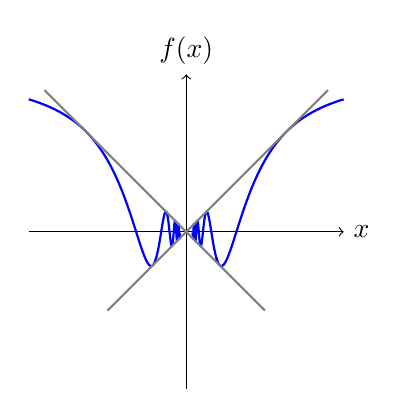
\begin{tikzpicture}[scale=2]
	\draw[->] (-1,0)--(1,0) node[right]{$x$};
	\draw[->] (0,-1)--(0,1) node[above]{$f(x)$};
	\draw[-,blue,thick,domain=-1:-0.19]plot[samples=400](\x,{\x*sin(180/(\x*pi))});
	\draw[-,blue,thick,domain=-0.2:-0.04]plot[samples=1000](\x,{\x*sin(180/(\x*pi))});
	\draw[-,blue,thick,domain=0.19:1]plot[samples=400](\x,{\x*sin(180/(\x*pi))});
	\draw[-,blue,thick,domain=0.04:0.2]plot[samples=1000](\x,{\x*sin(180/(\x*pi))});
	\draw[-,thick,gray,domain=-0.5:0.9] plot[smooth](\x,\x);
	\draw[-,thick,gray,domain=-0.9:0.5] plot[smooth](\x,-\x);
\end{tikzpicture}
\end{document}
\end{document}
    \end{tightcenter}
    
\end{solution}
除了使用夹逼准则以外,我们还可以利用极限的四则运算和复合来计算复杂函数的极限.
\begin{theorem}[0A.1.4 极限的四则运算]
    如果$f(x)$和$g(x)$满足
    \[\lim_{x\to a}f(x)=l_1\ \ \ \ \ \lim_{x\to a}g(x)=l_2\]
    那么我们有
    \[\lim_{x\to a}f(x)\pm g(x)=\l_1\pm l_2\]
    \[\lim_{x\to a}f(x)\cdot g(x)=l_1l_2\]
    \[\lim_{x\to a}\dfrac{f(x)}{g(x)}=\dfrac{l_1}{l_2}\left(l_2\neq0\right)\]
    即如果两个函数在某处的极限均存在,那么这两个函数的四则运算所得的函数在此处的极限亦存在,并且其值等于各自的极限值进行相应的四则运算的结果.
\end{theorem}
\begin{theorem}[0A.1.5 复合函数的极限]
    如果$\displaystyle\lim_{x\to a}f(x)=l$,而$g(x)$在$x=l$及其附近的区间上连续,那么
    \[\lim_{x\to a}g(f(x))=g(l)\]
    这就是说,如果复合函数的外部连续(这一条件是容易满足的),就可以先对内部求极限后代入外部函数从而得到总体的极限值.
\end{theorem}
上面两个定理的证明较为繁琐,因此你不必掌握它们的证明方法.总之,极限运算(在我们目前能接触到的函数中)%
是十分符合常理的.
\Section{0A.1 导数}
\Part{导数的简单定义}
\indent 出于简单考虑,我们不准备介绍极限的定义和严格定义导数的方法\footnote{尽管这一概念是高等数学的基础.}.%
或者更确切地说,这一章节的内容都是为了让你对微积分有一个简单的,偏向直观的了解,而非与那些性质古怪的函数打交道.
\begin{hint}
    本书所考虑的所有函数几乎都是光滑的.这在图像上表现为一条“看起来”光滑的曲线,没有间断的地方,没有粗糙的折点.%
    一个函数光滑意味着它具有良好的性质,我们可以不加考虑地对它进行求导,无需担心可能出现的差错或意外.
\end{hint}
正如前言中所说,人们是从物体的运动状态开始研究微积分的.在初中时,你应当学过简单的运动学知识:在一段时间$t$内,物体运动的距离\footnote{准确而言应当是位移.此处我们假定物体做直线运动,因而位移就与距离的数值相同.}%
$x$与$t$之比就是它在这段时间内的平均速度$v$,即
\[v=\dfrac xt\]
我们让这段时间从某一时间点$t_0$开始,并结束于$t_0+\Delta t$,在这段时间内物体运动的距离为$\Delta x$.于是这段时间内的平均速度为
\[\bar{v}=\dfrac{\Delta x}{\Delta t}\]
现在让$\Delta t$越来越小.在此过程中,物体的平均速度$\bar{v}$应当\tbf{趋近}于某一定值,这就是某一时间$t_0$时该物体的瞬时速度$v_0$,可以记为
\[v_0=\lim_{\Delta t\to 0}\dfrac{\Delta x}{\Delta t}\]
这就是导数的定义.上面的$\lim$代表limit,意为“极限”.由于本书并不打算涉及极限的定义,因此上述式子只需意会即可:%
某一时间$t_0$的瞬时速度$v_0$等于当$\Delta t$趋近于$0$时$\left(t_0,t_0+\Delta t\right)$时间段内的运动距离$\Delta x$与$\Delta t$之比值.\\
\indent 我们知道,速度即为运动距离对时间的变化率.上面的叙述就可以引出导数的(浅显而形象的)定义.
\begin{definition}[0A.1.1 导数]
    函数$y=f(x)$在$x=x_0$处的导数定义为
    \[f'\left(x_0\right)=\lim_{\Delta x\to 0}\dfrac{f\left(x+\Delta x\right)-f(x)}{\Delta x}\]
    在各点处的$f'\left(x_0\right)$亦可以构成一个新的函数,这一函数$f'(x)$记为$f(x)$的导函数.%
    今后,我们说某一函数的导数,一般就指其导函数.
\end{definition}
至此,基础的介绍就已经完结了\footnote{上述内容似有听君一席话如听一席话的感受,这实在是由于笔者不才而不能很好地介绍导数所致.}.%
如果你想对高等数学的内容有更加深入的了解,笔者建议你阅读普林斯顿微积分读本以获得对微积分的初步认识,然后再阅读各种高等数学书籍.\vspace{4pt}\\
\Part{常见函数的导数}
\indent 接下来,我们将从定义出发推导一些函数的导函数\footnote{这会不可避免地引入极限的四则运算,你只需意会即可.%
总之,尽管$\Delta x$在很多结果里都看似是$0$,但它总是不为$0$.我们需要思考的是当它接近$0$时整个式子所接近的值,%
这和直接把$\Delta x=0$代入是有区别的,毕竟分母不可能为$0$.},首先是简单的幂函数.
\begin{derivation}
    我们先从最简单的$f(x)=x$入手.我们有
    \[f'(x)=\lim_{\Delta x\to0}\dfrac{f(x+\Delta x)-f(x)}{\Delta x}
    =\lim_{\Delta x\to0}\dfrac{x+\Delta x-x}{\Delta x}=\lim_{\Delta x\to0}1=1\]
    因此$f(x)=x$的导函数处处为$1$.\\
    现在考虑$f(x)=x^2$.情况要稍微复杂一些.
    \[\begin{aligned}
        f'(x)
        &= \lim_{\Delta x\to0}\dfrac{f(x+\Delta x)-f(x)}{\Delta x}=\lim_{\Delta x\to0}\dfrac{(x+\Delta x)^2-x^2}{\Delta x} \\
        &= \lim_{\Delta x\to0}\dfrac{2x\Delta x-(\Delta x)^2}{\Delta x}=\lim_{\Delta x\to0}(2x+\Delta x)=2x
    \end{aligned}\]
    而$f(x)=\dfrac1x$也是相似的.
    \[\begin{aligned}
        f'(x)
        &= \lim_{\Delta x\to0}\dfrac{f(x+\Delta x)-f(x)}{\Delta x}=\lim_{\Delta x\to0}\dfrac{\frac{1}{x+\Delta x}-\frac1x}{\Delta x} \\
        &= \lim_{\Delta x\to0}\dfrac{1}{\Delta x}\cdot\dfrac{x-(x+\Delta x)}{x(x+\Delta x)} \\
        &= -\lim_{\Delta x\to0}\dfrac{1}{x^2+x\Delta x} \\
        &= -\dfrac1{x^2}
    \end{aligned}\]
    现在再来考虑$f(x)=\sqrt{x}$.我们有
    \[\begin{aligned}
        f'(x)
        &= \lim_{\Delta x\to0}\dfrac{f(x+\Delta x)-f(x)}{\Delta x}=\lim_{\Delta x\to0}\dfrac{\sqrt{x+\Delta x}-\sqrt{x}}{\Delta x} \\
        &= \lim_{\Delta x\to0}\dfrac{(x+\Delta x)-x}{\left(\sqrt{x+\Delta x}+\sqrt{x}\right)\Delta x} \\
        &= \lim_{\Delta x\to0}\dfrac{1}{\sqrt{x+\Delta x}+\sqrt{x}} \\
        &= \dfrac{1}{2\sqrt{x}}
    \end{aligned}\]
    我们可以归纳出以下结论:幂函数$f(x)=x^a$的导函数为$f'(x)=ax^{a-1}$.这一结论的严格证明过程请查阅资料.
\end{derivation}
\begin{theorem}[0A.1.2 幂函数的导数]
    幂函数$f(x)=x^a(a\in\R)$的导函数为$f'(x)=ax^{a-1}$.
\end{theorem}
接下来是常见的三角函数.在推到之前,我们需要知道一个重要极限.
\begin{theorem}[0A.1.3 重要极限I]
    我们有重要极限
    \[\lim_{x\to0}\dfrac{\sin x}{x}=1\]
    你可以自行查阅这一极限的证明方法.
\end{theorem}
\begin{derivation}
    先考虑$f(x)=\sin x$.我们有
    \[\begin{aligned}
        f'(x)
        &= \lim_{\Delta x\to0}\dfrac{f(x+\Delta x)-f(x)}{\Delta x}=\lim_{\Delta x\to0}\dfrac{\sin(x+\Delta x)-\sin{x}}{\Delta x} \\
        &= \lim_{\Delta x\to0}\dfrac{\sin x\cos\Delta x+\sin\Delta x\cos x-\sin x}{\Delta x} \\
        &= \lim_{\Delta x\to0}\dfrac{\sin x(1-\cos\Delta x)}{\Delta x}+\lim_{\Delta x\to0}\dfrac{\cos x\sin\Delta x}{\Delta x} \\
        &= 0+\cos x=\cos x
    \end{aligned}\]
    其中
\end{derivation}
\Part{导(函)数的运算法则}
\indent 导函数的运算法则是十分重要且基础的工具.
\begin{theorem}[0A.1.2]
    导函数的运算法则主要有以下几条.
    \begin{enumerate}[label=\tbf{\roman*.},topsep=0pt,parsep=0pt,itemsep=0pt,partopsep=0pt]
        \item \tbf{导数的加减法}\\如果$h(x)=f(x)\pm g(x)$,那么$h'(x)=f'(x)\pm g'(x)$.
        \item \tbf{导数的乘法}\\如果$h(x)=f(x)g(x)$,那么$h'(x)=f'(x)g(x)+f(x)g'(x)$.
        \item \tbf{导数的除法}\\如果$h(x)=f(x)$
        \item 如果$h(x)=f(g(x))$,那么$h'(x)$
    \end{enumerate}
\end{theorem}
\end{document}